\section{Quantum communication systems with PACSs}
    The effect of the use of PACS in an OOK communication system was extensively discussed in
    \cite{PACSDisc}. In this section the most important result will be reported and a BPSK
    system will be tested.

    \subsection{Quantum OOK}
    The use of PACS in an OOK system can significantly improve the performance. The MDEP, with
    thermal noise, is given by the Helstrom bound \ref{eq:HelstromBound}, where, for an OOK PACS
    system,
    \begin{equation}
        \Operator{\varXi}_0 =  \Operator{\varXi}_{\mathrm{th}}^{(0)}(0)
    \end{equation}
    \begin{equation*}
        \Operator{\varXi}_1 =  \Operator{\varXi}_{\mathrm{th}}^{(k)}(\mu).
    \end{equation*}
    It is useful, in order to evaluate the performance of the system, to introduce the mean number
    of photon $n_p$ in a quantum state $\Operator{\varXi}$, which is given by:
    \begin{equation}
        n_p = \tr{\Operator{\varXi}\Operator{A}^\dagger\Operator{A}}.
        \label{eq:genericnp}
    \end{equation}
    For a photon added coherent state, the equation \ref{eq:genericnp} becomes \cite{PACSDisc}:
    \begin{equation}
        n_p(\mu,\bar{n}) = \frac{N_{k+1}(\mu,\bar{n})}{N_k(\mu,\bar{n})}-1,
        \label{eq:np}
    \end{equation}
    where
    \begin{equation}
        N_k(\mu,\bar{n}) = \tr{(\Operator{A}^\dagger)^k \Operator{\varXi}_{\mathrm{th}}(\mu) \Operator{A}^k}.
    \end{equation}
    It is possible to observe that the minimum of $n_p$ is given by:
    \begin{equation}
        n_p(0,\bar{n}) = (k+1)(\bar{n}+1)-1.
        \label{eq:min_np}
    \end{equation}

    \begin{figure}[t]
        \begin{center}
            %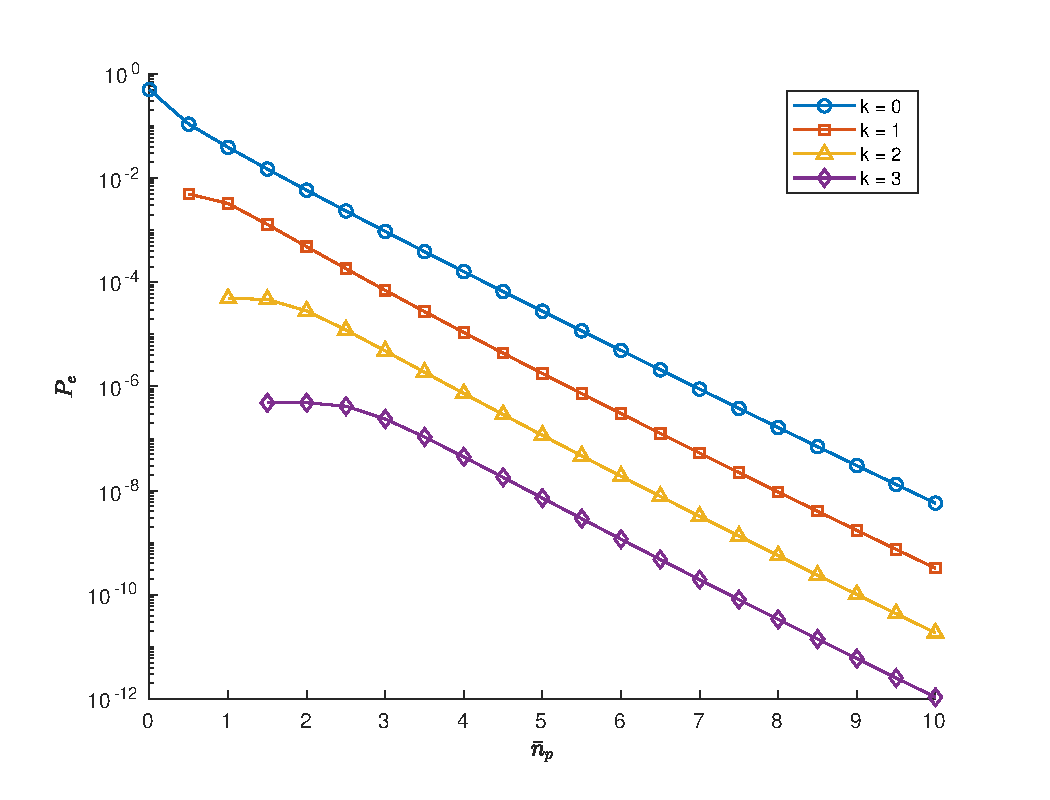
\includegraphics[width=0.8\textwidth]{fig3.1.eps}
            % This file was created by matlab2tikz.
%
%The latest updates can be retrieved from
%  http://www.mathworks.com/matlabcentral/fileexchange/22022-matlab2tikz-matlab2tikz
%where you can also make suggestions and rate matlab2tikz.
%
\definecolor{mycolor1}{rgb}{0.00000,0.44700,0.74100}%
\definecolor{mycolor2}{rgb}{0.85000,0.32500,0.09800}%
\definecolor{mycolor3}{rgb}{0.92900,0.69400,0.12500}%
\definecolor{mycolor4}{rgb}{0.49400,0.18400,0.55600}%
%
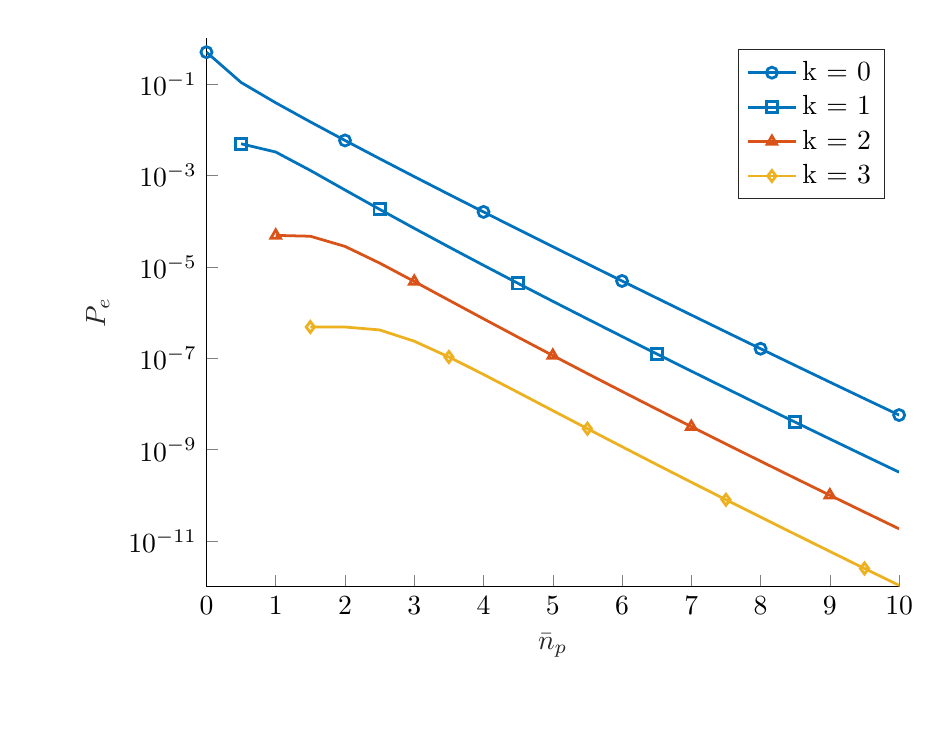
\begin{tikzpicture}
\begin{axis}[%
width=5.328in*0.65,
height=4.219in*0.65,
at={(0.894in,0.569in)},
scale only axis,
unbounded coords=jump,
xmin=0,
xmax=10,
xlabel style={font=\color{white!15!black}},
xlabel={$\bar{n}_p$},
ymode=log,
ymin=1e-12,
ymax=1,
yminorticks=true,
ylabel style={font=\color{white!15!black}},
ylabel={$P_e$},
axis background/.style={fill=white},
axis x line*=bottom,
axis y line*=left,
legend style={legend cell align=left, align=left, draw=white!15!black}
]
\addplot [color=mycolor1, line width=1.0pt, mark=o, mark options={solid, mycolor1}, mark repeat={4}]
  table[row sep=crcr]{%
0	0.5\\
0.5	0.108700458264773\\
1	0.0390589952204486\\
1.5	0.0149211944183797\\
2	0.00585810811660969\\
2.5	0.00234016700918788\\
3	0.000947208632045338\\
3.5	0.000387493710183651\\
4	0.000159914030711417\\
4.5	6.64741461101626e-05\\
5	2.77991876821981e-05\\
5.5	1.16842832866837e-05\\
6	4.93215909780353e-06\\
6.5	2.08982945676395e-06\\
7	8.88612131100253e-07\\
7.5	3.79192264921002e-07\\
8	1.62439465989372e-07\\
8.5	6.98919122021913e-08\\
9	3.02206709656971e-08\\
9.5	1.31382953405534e-08\\
10	5.74554720467191e-09\\
};
\addlegendentry{k = 0}

\addplot [color=mycolor2, line width=1.0pt, mark=square, mark options={solid, mycolor2},mark repeat={4}]
  table[row sep=crcr]{%
0	nan\\
0.5	0.00495049504950484\\
1	0.00326586474485635\\
1.5	0.00129261012790083\\
2	0.000482962413068555\\
2.5	0.000182311367178389\\
3	7.00429974659356e-05\\
3.5	2.73706279001473e-05\\
4	1.0858752113041e-05\\
4.5	4.36492362687613e-06\\
5	1.77429661629702e-06\\
5.5	7.2806225398514e-07\\
6	3.01146871883873e-07\\
6.5	1.25430517805558e-07\\
7	5.25760247560569e-08\\
7.5	2.21744258510626e-08\\
8	9.41026234713149e-09\\
8.5	4.01790212212205e-09\\
9	1.72544134535713e-09\\
9.5	7.44933115193191e-10\\
10	3.23308935179512e-10\\
};
\addlegendentry{k = 1}

\addplot [color=mycolor3, line width=1.0pt, mark=triangle, mark options={solid, mycolor3},mark repeat={4}]
  table[row sep=crcr]{%
0	nan\\
0.5	nan\\
1	4.90148024704373e-05\\
1.5	4.69619801757304e-05\\
2	2.81400977715229e-05\\
2.5	1.21516986146819e-05\\
3	4.80779254996566e-06\\
3.5	1.87442312044039e-06\\
4	7.3327408445234e-07\\
4.5	2.89379331441797e-07\\
5	1.1537747546253e-07\\
5.5	4.64728403537507e-08\\
6	1.88977288262393e-08\\
6.5	7.75273512054753e-09\\
7	3.20750448423723e-09\\
7.5	1.33800148738317e-09\\
8	5.62493496225613e-10\\
8.5	2.3806545623728e-10\\
9	1.01301078636595e-10\\
9.5	4.33071356553683e-11\\
10	1.86188842121737e-11\\
};
\addlegendentry{k = 2}

\addplot [color=mycolor4, line width=1.0pt, mark=diamond, mark options={solid, mycolor4},mark repeat={4}]
  table[row sep=crcr]{%
0	nan\\
0.5	nan\\
1	nan\\
1.5	4.85295073904268e-07\\
2	4.85188186960528e-07\\
2.5	4.18524906453666e-07\\
3	2.37374074840702e-07\\
3.5	1.07056314813114e-07\\
4	4.441501411101e-08\\
4.5	1.79385633014562e-08\\
5	7.1959126435317e-09\\
5.5	2.89084600701983e-09\\
6	1.16757170598447e-09\\
6.5	4.75056216586722e-10\\
7	1.94958549304403e-10\\
7.5	8.07277023007202e-11\\
8	3.36927152844169e-11\\
8.5	1.41446854229343e-11\\
9	5.96345195447157e-12\\
9.5	2.52742271555917e-12\\
10	1.08146824828736e-12\\
};
\addlegendentry{k = 3}

\end{axis}

\begin{axis}[%
width=6.875in*0.65,
height=5.177in*0.65,
at={(0in,0in)},
scale only axis,
xmin=0,
xmax=1,
ymin=0,
ymax=1,
axis line style={draw=none},
ticks=none,
axis x line*=bottom,
axis y line*=left
]
\end{axis}
\end{tikzpicture}%
            \caption{MDEP for PACS QOOK as function of $\bar{n}_p$ with: $k=0,1,2,3$; $\bar{n}=10^{-2}$; $p_0=p_1=1/2$}
            \label{fig:3.1}
        \end{center}
    \end{figure}
    The MDEP of a quantum OOK system with PACS in function of $\bar{n}_p$ is represented in the figure
    \ref{fig:3.1}. The parameter $\bar{n}_p$ represents the mean number of photons in the system and it is 
    defined as
    \begin{equation*}
        \bar{n}_p=\frac{1}{2} \left(n_{p0}+n_{p1}\right)
    \end{equation*}
    where $n_{pi}$ is the mean number of photons in the state $\Operator{\varXi}_i$.
    The parameter $\bar{n}_p$ is equal to $n_p/2$ for OOK systems and to the average of the $n_p$ for 
    each state for the BPSK system.
    In the y-axes there are the MDEP ($P_e$). The plot was obtained for equiprobable symbols and 
    mean number of thermal photons $\bar{n}=10^{-2}$.  
    The argument of the trace norm $\norm{\cdot}_1$ in the Helstrom bound 
    \ref{eq:HelstromBound}, is an operator in an infinite dimensional Hilbert space; for the 
    simulation, it has been approximated in $N=30$ dimension.
    We can observe that the photon addition improves significantly the performance in terms
    of error probability. Incrasing the value of the parameter $k$ the MDEP of the system 
    transate; the error probability, for the same energy-level, is lower if $k$ is bigger.
    We can notice too that the graphs do not start all from $0$. This is because the minimum
    mean number of photons in a photon added state is not always $0$ as it possible to see in 
    equation \ref{eq:min_np}.  

    \subsection{Quantum BPSK}
    It can be interesting to assess the effect of photon addition in a quantum BPSK system.
    The constellation is given, for a PACS BPSK, by:
    \begin{subequations}\begin{align}
        \Operator{\varXi}_0 &=  \Operator{\varXi}_{\mathrm{th}}^{(k)}(-\mu)\\
        \Operator{\Xi}_1 &=  \Operator{\varXi}_{\mathrm{th}}^{(k)}(\mu).
    \end{align}\end{subequations}
    %
    In absence of noise ($\bar{n}=0$), the MDEP is given by formula \ref{eq:HelstromBPure} where
    \begin{subequations}
        \begin{align}
            \ket{\psi_0}&=\ket*{-\mu^{(k)}},\\
            \ket{\psi_1}&=\ket*{\mu^{(k)}}.
        \end{align}
    \end{subequations}
    %
    The inner product is given, in closed form, by \cite{PACSDisc}:
    \begin{equation}
        \braket*{-\mu^{(k)}}{\mu^{(k)}} = \frac{L_k(\absolutevalue{\mu}^2)}{L_k(-\absolutevalue{\mu}^2)}
        e^{-2\absolutevalue{\mu}^2},
        \label{eq:innerp_nonNoise}
    \end{equation}
    where $L_k(x)$ is the Laguerre polynomial of parameter $k$, evaluate in $x$.
    \begin{figure}[t]
        \begin{subfigure}{0.5\textwidth}
            %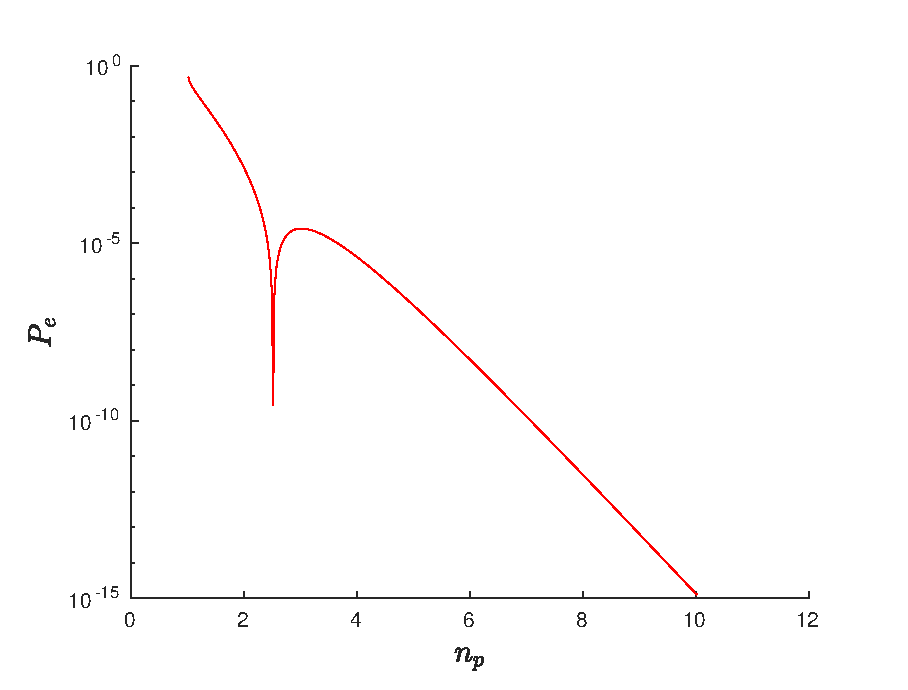
\includegraphics[width=\linewidth]{fig3.2a.eps}
            % This file was created by matlab2tikz.
%
%The latest updates can be retrieved from
%  http://www.mathworks.com/matlabcentral/fileexchange/22022-matlab2tikz-matlab2tikz
%where you can also make suggestions and rate matlab2tikz.
%
\begin{tikzpicture}

\begin{axis}[%
width=4.521in*0.45,
height=3.566in*0.45,
at={(0.758in,0.481in)},
scale only axis,
unbounded coords=jump,
xmin=0,
xmax=12,
xlabel style={font=\color{white!15!black}},
xlabel={$n_p$},
ymode=log,
ymin=1e-15,
ymax=1,
yminorticks=true,
ylabel style={font=\color{white!15!black}},
ylabel={$P_e$},
axis background/.style={fill=white},
axis x line*=bottom,
axis y line*=left
]
\addplot [color=red, forget plot, line width=1.0pt]
  table[row sep=crcr]{%
0	1\\
0.02	nan\\
0.04	nan\\
0.06	nan\\
0.08	nan\\
0.1	nan\\
0.12	nan\\
0.14	nan\\
0.16	nan\\
0.18	nan\\
0.2	nan\\
0.22	nan\\
0.24	nan\\
0.26	nan\\
0.28	nan\\
0.3	nan\\
0.32	nan\\
0.34	nan\\
0.36	nan\\
0.38	nan\\
0.4	nan\\
0.42	nan\\
0.44	nan\\
0.46	nan\\
0.48	nan\\
0.5	nan\\
0.52	nan\\
0.54	nan\\
0.56	nan\\
0.58	nan\\
0.6	nan\\
0.62	nan\\
0.64	nan\\
0.66	nan\\
0.68	nan\\
0.7	nan\\
0.72	nan\\
0.74	nan\\
0.76	nan\\
0.78	nan\\
0.8	nan\\
0.82	nan\\
0.84	nan\\
0.86	nan\\
0.88	nan\\
0.9	nan\\
0.92	nan\\
0.94	nan\\
0.96	nan\\
0.98	nan\\
1	nan\\
1.02	0.5\\
1.04	0.472399701057977\\
1.06	0.357983234584284\\
1.08	0.307507799177868\\
1.1	0.26599128917996\\
1.12	0.235397163233556\\
1.14	0.209279937900031\\
1.16	0.187232467240902\\
1.18	0.168833144138996\\
1.2	0.15158247927088\\
1.22	0.136460804349467\\
1.24	0.122354552686578\\
1.26	0.110943447278033\\
1.28	0.100277610011171\\
1.3	0.0903427728698788\\
1.32	0.0818057131680995\\
1.34	0.0738601967962477\\
1.36	0.067080892579425\\
1.38	0.0602166128167249\\
1.4	0.0543936491038224\\
1.42	0.0494744894265663\\
1.44	0.0444585211157397\\
1.46	0.0402425031269407\\
1.48	0.0363392303947938\\
1.5	0.0327341394723772\\
1.52	0.0294125498545432\\
1.54	0.0263597482547049\\
1.56	0.0238299165445917\\
1.58	0.0212475048666858\\
1.6	0.0191175222188837\\
1.62	0.0171608092274059\\
1.64	0.0153672521330726\\
1.66	0.0137269658182734\\
1.68	0.0122303219697235\\
1.7	0.0108679740170279\\
1.72	0.00976242258067622\\
1.74	0.00862933146911044\\
1.76	0.00771395212857762\\
1.78	0.00678007951997928\\
1.8	0.00602921274897855\\
1.82	0.00534749784926047\\
1.84	0.00472996050928637\\
1.86	0.00413884603820058\\
1.88	0.0036389564997123\\
1.9	0.00318945202436305\\
1.92	0.0028102088674179\\
1.94	0.00244704015090319\\
1.96	0.00212303902261424\\
1.98	0.00183482081201486\\
2	0.00160948401679273\\
2.02	0.00137997049047073\\
2.04	0.00118956676812737\\
2.06	0.00102093436399392\\
2.08	0.000872072832805881\\
2.1	0.000741120598089617\\
2.12	0.000633530054419074\\
2.14	0.000532414004556503\\
2.16	0.000444493365702903\\
2.18	0.000373127818625141\\
2.2	0.000311032842465642\\
2.22	0.000257259333784232\\
2.24	0.000207887668100259\\
2.26	0.000168651891669258\\
2.28	0.000135274598132118\\
2.3	0.00010708720509206\\
2.32	8.34800194294827e-05\\
2.34	6.51746714170343e-05\\
2.36	4.88797710067046e-05\\
2.38	3.56834113079962e-05\\
2.4	2.51720831376812e-05\\
2.42	1.74900742125894e-05\\
2.44	1.1534198714358e-05\\
2.46	6.77424237466306e-06\\
2.48	3.66023472747612e-06\\
2.5	1.60604061122394e-06\\
2.52	3.82699611611859e-07\\
2.54	3.36912281406754e-09\\
2.56	2.15313998297439e-07\\
2.58	9.0092844268197e-07\\
2.6	1.95716900108778e-06\\
2.62	3.18325902654015e-06\\
2.64	4.83437297199574e-06\\
2.66	6.37823821686423e-06\\
2.68	8.12932535254607e-06\\
2.7	9.91460547444811e-06\\
2.72	1.15573462030616e-05\\
2.74	1.32993609222032e-05\\
2.76	1.48490515805566e-05\\
2.78	1.6443531399124e-05\\
2.8	1.78225188985914e-05\\
2.82	1.91013611508528e-05\\
2.84	2.02722099845731e-05\\
2.86	2.14125652719943e-05\\
2.88	2.23435969195496e-05\\
2.9	2.31565610588902e-05\\
2.92	2.38517688561646e-05\\
2.94	2.44308602199705e-05\\
2.96	2.48965896211262e-05\\
2.98	2.52526333738845e-05\\
3	2.55034168804569e-05\\
3.02	2.56539604011063e-05\\
3.04	2.57085727939921e-05\\
3.06	2.56825909074609e-05\\
3.08	2.55731959089012e-05\\
3.1	2.53865606292814e-05\\
3.12	2.51529495969849e-05\\
3.14	2.48644718423008e-05\\
3.16	2.44927751494872e-05\\
3.18	2.40674950605646e-05\\
3.2	2.36356278071059e-05\\
3.22	2.31681021719554e-05\\
3.24	2.26223943989301e-05\\
3.26	2.2093839465942e-05\\
3.28	2.15421925337522e-05\\
3.3	2.09711379927646e-05\\
3.32	2.03841608488742e-05\\
3.34	1.97295132032815e-05\\
3.36	1.91196068240473e-05\\
3.38	1.85032584362754e-05\\
3.4	1.78831174386662e-05\\
3.42	1.72616328440456e-05\\
3.44	1.6641057451694e-05\\
3.46	1.60234529889558e-05\\
3.48	1.54661550202939e-05\\
3.5	1.48592830506722e-05\\
3.52	1.42603515138617e-05\\
3.54	1.36707378644019e-05\\
3.56	1.31438413250584e-05\\
3.58	1.25752809384538e-05\\
3.6	1.20191837034711e-05\\
3.62	1.15251406966888e-05\\
3.64	1.09949833971834e-05\\
3.66	1.05255764755174e-05\\
3.68	1.00234781867381e-05\\
3.7	9.58028685626999e-06\\
3.72	9.10762996930714e-06\\
3.74	8.69161100347515e-06\\
3.76	8.28870977404028e-06\\
3.78	7.86072089425938e-06\\
3.8	7.48545582957005e-06\\
3.82	7.12329941227052e-06\\
3.84	6.77416475253212e-06\\
3.86	6.40501080761968e-06\\
3.88	6.0827893155202e-06\\
3.9	5.77311551952508e-06\\
3.92	5.47578188991871e-06\\
3.94	5.19055937303614e-06\\
3.96	4.91720013240382e-06\\
3.98	4.65544011912788e-06\\
4	4.40500147547151e-06\\
4.02	4.16559477561806e-06\\
4.04	3.93692110922661e-06\\
4.06	3.71867401188775e-06\\
4.08	3.51054124908545e-06\\
4.1	3.33160810583877e-06\\
4.12	3.1418188061183e-06\\
4.14	2.96122031268053e-06\\
4.16	2.7894923582128e-06\\
4.18	2.64225763085824e-06\\
4.2	2.48650592976629e-06\\
4.22	2.33870550919724e-06\\
4.24	2.21222658025599e-06\\
4.26	2.0786812897633e-06\\
4.28	1.96453803136265e-06\\
4.3	1.84415963971896e-06\\
4.32	1.74139010983287e-06\\
4.34	1.63313089546202e-06\\
4.36	1.54081241204862e-06\\
4.38	1.44367094412345e-06\\
4.4	1.36092452862613e-06\\
4.42	1.27817808270869e-06\\
4.44	1.19994328223738e-06\\
4.46	1.12980019706388e-06\\
4.48	1.0597632829068e-06\\
4.5	9.93646884384081e-07\\
4.52	9.34456640067083e-07\\
4.54	8.78462594666729e-07\\
4.56	8.25515935110044e-07\\
4.58	7.72775243351731e-07\\
4.6	7.23107359767994e-07\\
4.62	6.78746309934475e-07\\
4.64	6.36875023218852e-07\\
4.66	5.97370669985775e-07\\
4.68	5.60115256176275e-07\\
4.7	5.2499552410934e-07\\
4.72	4.91902847454817e-07\\
4.74	4.60733121321333e-07\\
4.76	4.31386648236387e-07\\
4.78	4.03768021295381e-07\\
4.8	3.77786004479574e-07\\
4.82	3.53353410753598e-07\\
4.84	3.31625796101687e-07\\
4.86	3.11138908359876e-07\\
4.88	2.9072807899988e-07\\
4.9	2.71563803166952e-07\\
4.92	2.5357691213479e-07\\
4.94	2.38523682916103e-07\\
4.96	2.22583676767751e-07\\
4.98	2.07639469451681e-07\\
5	1.94388511010057e-07\\
5.02	1.81929371900758e-07\\
5.04	1.6955217713166e-07\\
5.06	1.58588868259812e-07\\
5.08	1.48291097012976e-07\\
5.1	1.38071630850778e-07\\
5.12	1.29545061733349e-07\\
5.14	1.20543526771488e-07\\
5.16	1.13037982363284e-07\\
5.18	1.05119423554623e-07\\
5.2	9.85210918402757e-08\\
5.22	9.15640828713649e-08\\
5.24	8.57706541901315e-08\\
5.26	7.99942483920013e-08\\
5.28	7.45858069750582e-08\\
5.3	6.981204470069e-08\\
5.32	6.50565297188876e-08\\
5.34	6.06079995635334e-08\\
5.36	5.66849587824159e-08\\
5.38	5.27803336591859e-08\\
5.4	4.91310470640549e-08\\
5.42	4.59156345167244e-08\\
5.44	4.29001787427552e-08\\
5.46	3.99022951902417e-08\\
5.48	3.7103730310406e-08\\
5.5	3.46406836548852e-08\\
5.52	3.23333284590888e-08\\
5.54	3.01723903084472e-08\\
5.56	2.81491071563167e-08\\
5.58	2.61409498492071e-08\\
5.6	2.43759617490902e-08\\
5.62	2.26251332668959e-08\\
5.64	2.10871596295625e-08\\
5.66	1.96490654857939e-08\\
5.68	1.83047088597732e-08\\
5.7	1.70483006600719e-08\\
5.72	1.58743860834143e-08\\
5.74	1.47778269621313e-08\\
5.76	1.37537852218372e-08\\
5.78	1.28555524558926e-08\\
5.8	1.19592910574617e-08\\
5.82	1.11229191412932e-08\\
5.84	1.03898237235889e-08\\
5.86	9.65885738057892e-09\\
5.88	8.97723478887613e-09\\
5.9	8.34178265352037e-09\\
5.92	7.74952008120167e-09\\
5.94	7.23100712640701e-09\\
5.96	6.74582234516663e-09\\
5.98	6.26272600445787e-09\\
6	5.81289277823416e-09\\
6.02	5.41943612208939e-09\\
6.04	5.05159647445907e-09\\
6.06	4.68567518119301e-09\\
6.08	4.3452702547242e-09\\
6.1	4.06700612076705e-09\\
6.12	3.76993997130981e-09\\
6.14	3.49378048714044e-09\\
6.16	3.2681805595125e-09\\
6.18	3.02749281200221e-09\\
6.2	2.8173945954002e-09\\
6.22	2.62135751993853e-09\\
6.24	2.4267338694095e-09\\
6.26	2.26791135871096e-09\\
6.28	2.0986464233097e-09\\
6.3	1.96057553525364e-09\\
6.32	1.81348769334733e-09\\
6.34	1.69355673929061e-09\\
6.36	1.5658463969892e-09\\
6.38	1.46175838100504e-09\\
6.4	1.35096428488524e-09\\
6.42	1.26070076600371e-09\\
6.44	1.17045101388769e-09\\
6.46	1.08645054064382e-09\\
6.48	1.01332026103407e-09\\
6.5	9.35557076253701e-10\\
6.52	8.72267758023071e-10\\
6.54	8.09049716110621e-10\\
6.56	7.50268291938028e-10\\
6.58	6.99143354321308e-10\\
6.6	6.48105291656265e-10\\
6.62	6.00677341200395e-10\\
6.64	5.59450652470872e-10\\
6.66	5.20966325634475e-10\\
6.68	4.82576312244021e-10\\
6.7	4.46929548925112e-10\\
6.72	4.15967038591702e-10\\
6.74	3.87084975184138e-10\\
6.76	3.58295337843373e-10\\
6.78	3.31583649426648e-10\\
6.8	3.08399361603762e-10\\
6.82	2.86788537362526e-10\\
6.84	2.66647870450498e-10\\
6.86	2.47880549419932e-10\\
6.88	2.29193941603256e-10\\
6.9	2.12989736958491e-10\\
6.92	1.96861194012854e-10\\
6.94	1.82880433019506e-10\\
6.96	1.69864511345708e-10\\
6.98	1.57749036056032e-10\\
7	1.46473555506788e-10\\
7.02	1.35981725879475e-10\\
7.04	1.26220645046971e-10\\
7.06	1.17141019106981e-10\\
7.08	1.08696718292833e-10\\
7.1	1.00844610440021e-10\\
7.12	9.35444499639004e-11\\
7.14	8.67585447927866e-11\\
7.16	8.04517563679497e-11\\
7.18	7.45912775990121e-11\\
7.2	6.91464108193429e-11\\
7.22	6.40885677860581e-11\\
7.24	5.93910476354154e-11\\
7.26	5.50288703493607e-11\\
7.28	5.12582198908262e-11\\
7.3	4.74784656034899e-11\\
7.32	4.42123004873451e-11\\
7.34	4.09393630107502e-11\\
7.36	3.79025144603418e-11\\
7.38	3.50853235353554e-11\\
7.4	3.24721916022952e-11\\
7.42	3.0215996371652e-11\\
7.44	2.81126233403484e-11\\
7.46	2.60068078183906e-11\\
7.48	2.40549247187971e-11\\
7.5	2.23706053681383e-11\\
7.52	2.06851757944548e-11\\
7.54	1.92312277214057e-11\\
7.56	1.77768355591468e-11\\
7.58	1.65225610970765e-11\\
7.6	1.53546619863221e-11\\
7.62	1.41869294090213e-11\\
7.64	1.31058497387926e-11\\
7.66	1.21741505765272e-11\\
7.68	1.13071774165974e-11\\
7.7	1.04407593681799e-11\\
7.72	9.69441193987564e-12\\
7.74	9.00018948257753e-12\\
7.76	8.35448377145553e-12\\
7.78	7.75407515973825e-12\\
7.8	7.15455472644067e-12\\
7.82	6.63846755344366e-12\\
7.84	6.15879569565436e-12\\
7.86	5.71298564011613e-12\\
7.88	5.29870591847725e-12\\
7.9	4.88531437525808e-12\\
7.92	4.55618875960795e-12\\
7.94	4.19952961294712e-12\\
7.96	3.89283050239442e-12\\
7.98	3.60800278542683e-12\\
8	3.34360317211235e-12\\
8.02	3.09813286136773e-12\\
8.04	2.87031509671465e-12\\
8.06	2.65887312167479e-12\\
8.08	2.46264120207229e-12\\
8.1	2.280620137185e-12\\
8.12	2.12430073531777e-12\\
8.14	1.9551027463649e-12\\
8.16	1.82065473808279e-12\\
8.18	1.68515201792729e-12\\
8.2	1.55953028269096e-12\\
8.22	1.44312339855901e-12\\
8.24	1.33515420941421e-12\\
8.26	1.24256160916048e-12\\
8.28	1.14935838624319e-12\\
8.3	1.06292752377612e-12\\
8.32	9.88875648033627e-13\\
8.34	9.14324171930048e-13\\
8.36	8.45268299798363e-13\\
8.38	7.81319453579954e-13\\
8.4	7.26474436163471e-13\\
8.42	6.71351862990832e-13\\
8.44	6.24111873293032e-13\\
8.46	5.76594327839075e-13\\
8.48	5.32629496063919e-13\\
8.5	4.94992935529126e-13\\
8.52	4.57078819238177e-13\\
8.54	4.24660306919122e-13\\
8.56	3.92075261146374e-13\\
8.58	3.64208663228283e-13\\
8.6	3.36175531856497e-13\\
8.62	3.12139203373363e-13\\
8.64	2.88047363738997e-13\\
8.66	2.674527266322e-13\\
8.68	2.48245868306185e-13\\
8.7	2.28983498828939e-13\\
8.72	2.12552198064486e-13\\
8.74	1.96009874997571e-13\\
8.76	1.81854531433601e-13\\
8.78	1.68698388591793e-13\\
8.8	1.56485935320916e-13\\
8.82	1.44273482050039e-13\\
8.84	1.33781874467331e-13\\
8.86	1.24067423001861e-13\\
8.88	1.1429746038516e-13\\
8.9	1.05970787700471e-13\\
8.92	9.82547376793264e-14\\
8.94	9.10382880192628e-14\\
8.96	8.43769498715119e-14\\
8.98	7.82152120848423e-14\\
9	7.19979631469414e-14\\
9.02	6.67244037799719e-14\\
9.04	6.178391132039e-14\\
9.06	5.72319969194268e-14\\
9.08	5.30131494258512e-14\\
9.1	4.90718576884319e-14\\
9.12	4.54636328584002e-14\\
9.14	4.20774526332934e-14\\
9.16	3.8968828164343e-14\\
9.18	3.60822483003176e-14\\
9.2	3.3362201889986e-14\\
9.22	3.08642000845794e-14\\
9.24	2.85882428840978e-14\\
9.26	2.64233079860787e-14\\
9.28	2.44804176929847e-14\\
9.3	2.26485497023532e-14\\
9.32	2.09277040141842e-14\\
9.34	1.94844140821715e-14\\
9.36	1.79856129989275e-14\\
9.38	1.66533453693773e-14\\
9.4	1.53765888910584e-14\\
9.42	1.4210854715202e-14\\
9.44	1.31561428418081e-14\\
9.46	1.21569421196455e-14\\
9.48	1.13242748511766e-14\\
9.5	1.04360964314765e-14\\
9.52	9.65894031423886e-15\\
9.54	8.99280649946377e-15\\
9.56	8.27116153345742e-15\\
9.58	7.66053886991358e-15\\
9.6	7.04991620636974e-15\\
9.62	6.60582699651968e-15\\
9.64	6.0507154842071e-15\\
9.66	5.6621374255883e-15\\
9.68	5.21804821573824e-15\\
9.7	4.82947015711943e-15\\
9.72	4.49640324973188e-15\\
9.74	4.10782519111308e-15\\
9.76	3.83026943495679e-15\\
9.78	3.5527136788005e-15\\
9.8	3.27515792264421e-15\\
9.82	3.05311331771918e-15\\
9.84	2.77555756156289e-15\\
9.86	2.60902410786912e-15\\
9.88	2.38697950294409e-15\\
9.9	2.22044604925031e-15\\
9.92	2.05391259555654e-15\\
9.94	1.88737914186277e-15\\
9.96	1.77635683940025e-15\\
9.98	1.60982338570648e-15\\
10	1.49880108324396e-15\\
10.02	1.38777878078145e-15\\
};
\end{axis}

\begin{axis}[%
width=5.833in*0.45,
height=4.375in*0.45,
at={(0in,0in)},
scale only axis,
xmin=0,
xmax=1,
ymin=0,
ymax=1,
axis line style={draw=none},
ticks=none,
axis x line*=bottom,
axis y line*=left
]
\end{axis}
\end{tikzpicture}%
            \caption{$k=1$}
        \end{subfigure}
        %\hspace*{fill}
        \begin{subfigure}{0.5\textwidth}
            %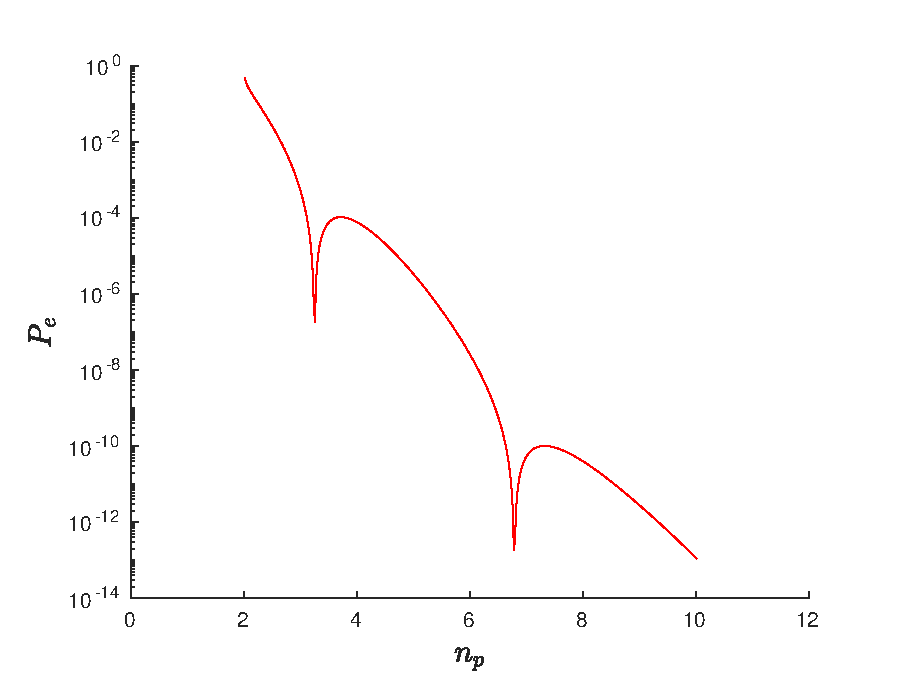
\includegraphics[width=\linewidth]{fig3.2b.eps}
            % This file was created by matlab2tikz.
%
%The latest updates can be retrieved from
%  http://www.mathworks.com/matlabcentral/fileexchange/22022-matlab2tikz-matlab2tikz
%where you can also make suggestions and rate matlab2tikz.
%
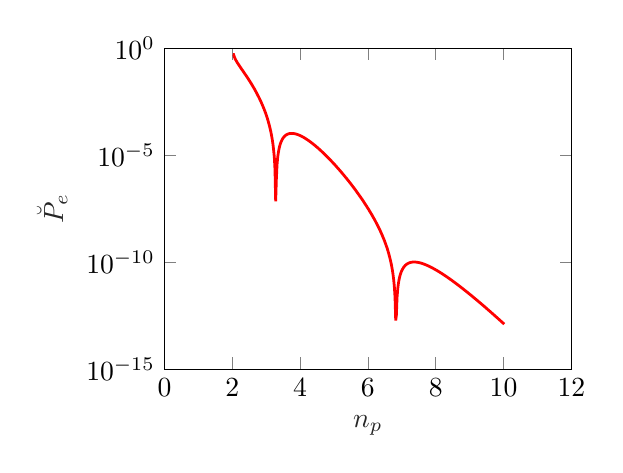
\begin{tikzpicture}

\begin{axis}[%
width=4.521in*0.45,
height=3.566in*0.45,
at={(0.758in,0.481in)},
scale only axis,
unbounded coords=jump,
xmin=0,
xmax=12,
xlabel style={font=\color{white!15!black}},
xlabel={$n_p$},
ymode=log,
ymin=1e-15,
ymax=1,
yminorticks=true,
ylabel style={font=\color{white!15!black}},
ylabel={$\breve{P}_e$},
axis background/.style={fill=white},
%axis x line*=bottom,
%axis y line*=left
]
\addplot [color=red, forget plot, line width=1.0pt]
  table[row sep=crcr]{%
0	1\\
0.02	nan\\
0.04	nan\\
0.06	nan\\
0.08	nan\\
0.1	nan\\
0.12	nan\\
0.14	nan\\
0.16	nan\\
0.18	nan\\
0.2	nan\\
0.22	nan\\
0.24	nan\\
0.26	nan\\
0.28	nan\\
0.3	nan\\
0.32	nan\\
0.34	nan\\
0.36	nan\\
0.38	nan\\
0.4	nan\\
0.42	nan\\
0.44	nan\\
0.46	nan\\
0.48	nan\\
0.5	nan\\
0.52	nan\\
0.54	nan\\
0.56	nan\\
0.58	nan\\
0.6	nan\\
0.62	nan\\
0.64	nan\\
0.66	nan\\
0.68	nan\\
0.7	nan\\
0.72	nan\\
0.74	nan\\
0.76	nan\\
0.78	nan\\
0.8	nan\\
0.82	nan\\
0.84	nan\\
0.86	nan\\
0.88	nan\\
0.9	nan\\
0.92	nan\\
0.94	nan\\
0.96	nan\\
0.98	nan\\
1	nan\\
1.02	nan\\
1.04	nan\\
1.06	nan\\
1.08	nan\\
1.1	nan\\
1.12	nan\\
1.14	nan\\
1.16	nan\\
1.18	nan\\
1.2	nan\\
1.22	nan\\
1.24	nan\\
1.26	nan\\
1.28	nan\\
1.3	nan\\
1.32	nan\\
1.34	nan\\
1.36	nan\\
1.38	nan\\
1.4	nan\\
1.42	nan\\
1.44	nan\\
1.46	nan\\
1.48	nan\\
1.5	nan\\
1.52	nan\\
1.54	nan\\
1.56	nan\\
1.58	nan\\
1.6	nan\\
1.62	nan\\
1.64	nan\\
1.66	nan\\
1.68	nan\\
1.7	nan\\
1.72	nan\\
1.74	nan\\
1.76	nan\\
1.78	nan\\
1.8	nan\\
1.82	nan\\
1.84	nan\\
1.86	nan\\
1.88	nan\\
1.9	nan\\
1.92	nan\\
1.94	nan\\
1.96	nan\\
1.98	nan\\
2	nan\\
2.02	0.5\\
2.04	0.5\\
2.06	0.3995486967565\\
2.08	0.331704531005947\\
2.1	0.286666971066393\\
2.12	0.251397256259136\\
2.14	0.221635982935945\\
2.16	0.196875556325859\\
2.18	0.176576485000044\\
2.2	0.157584967708243\\
2.22	0.142359394786826\\
2.24	0.126963768635949\\
2.26	0.114823798343439\\
2.28	0.102495467571005\\
2.3	0.0929383598487139\\
2.32	0.0831603206604107\\
2.34	0.074921311652674\\
2.36	0.0672821296493985\\
2.38	0.0602221018217888\\
2.4	0.0543448419737018\\
2.42	0.0489014184202455\\
2.44	0.0438738674007432\\
2.46	0.0392436388497789\\
2.48	0.0349917461486886\\
2.5	0.0310989102323145\\
2.52	0.0279243324786344\\
2.54	0.0246566682395089\\
2.56	0.0220070002129971\\
2.58	0.0195832098212382\\
2.6	0.0172405534724516\\
2.62	0.015240892011149\\
2.64	0.0134271714466244\\
2.66	0.01188462036823\\
2.68	0.0103961116588897\\
2.7	0.00905810656572942\\
2.72	0.00793039848272814\\
2.74	0.00691615866777207\\
2.76	0.00594974547556787\\
2.78	0.00519426587332583\\
2.8	0.00447065146517356\\
2.82	0.00382859586080297\\
2.84	0.00329674026011295\\
2.86	0.00279283971228139\\
2.88	0.00235105102899585\\
2.9	0.00198957280257689\\
2.92	0.0016726158165779\\
2.94	0.00139599121997341\\
2.96	0.00115578585448234\\
2.98	0.000948354652840377\\
3	0.000770312222623748\\
3.02	0.000618523732803133\\
3.04	0.000490095217214159\\
3.06	0.000382363405293407\\
3.08	0.000292885185846692\\
3.1	0.000224187049997215\\
3.12	0.000163777686606414\\
3.14	0.000118700047310016\\
3.16	8.04282095006048e-05\\
3.18	5.31254108838697e-05\\
3.2	3.26185302539916e-05\\
3.22	1.6995049294366e-05\\
3.24	8.1128488990112e-06\\
3.26	2.13187516551194e-06\\
3.28	6.88029047624106e-08\\
3.3	7.24374986382781e-07\\
3.32	3.54753374604e-06\\
3.34	8.05527932357109e-06\\
3.36	1.33466644199332e-05\\
3.38	1.99607138571811e-05\\
3.4	2.71846837265333e-05\\
3.42	3.47495029751621e-05\\
3.44	4.18382779365789e-05\\
3.46	4.94545149719583e-05\\
3.48	5.62942704171454e-05\\
3.5	6.33779358619191e-05\\
3.52	7.00240807412489e-05\\
3.54	7.570324547157e-05\\
3.56	8.08982915437295e-05\\
3.58	8.55775360911748e-05\\
3.6	9.00416624860512e-05\\
3.62	9.35936247979385e-05\\
3.64	9.6598721924801e-05\\
3.66	9.90635414040431e-05\\
3.68	0.000101000736447365\\
3.7	0.000102524539730031\\
3.72	0.000103423922654555\\
3.74	0.000103842610198968\\
3.76	0.000103882316017101\\
3.78	0.000103515220417627\\
3.8	0.000102771666713353\\
3.82	0.000101682676166781\\
3.84	0.000100279503038092\\
3.86	9.87438337359814e-05\\
3.88	9.68250215683253e-05\\
3.9	9.46811938021264e-05\\
3.92	9.25431394562248e-05\\
3.94	9.00481316531421e-05\\
3.96	8.76341504017497e-05\\
3.98	8.48859185277329e-05\\
4	8.22813458992155e-05\\
4.02	7.93678247413276e-05\\
4.04	7.66483559924147e-05\\
4.06	7.3646638171998e-05\\
4.08	7.08778646119623e-05\\
4.1	6.81057385766293e-05\\
4.12	6.53418674217976e-05\\
4.14	6.25968037595293e-05\\
4.16	5.96348103363287e-05\\
4.18	5.69587086937662e-05\\
4.2	5.43277317224256e-05\\
4.22	5.17484955028791e-05\\
4.24	4.92267635868182e-05\\
4.26	4.67674941659335e-05\\
4.28	4.43748881284178e-05\\
4.3	4.20524374896147e-05\\
4.32	3.98029737492256e-05\\
4.34	3.762871578461e-05\\
4.36	3.57187802187409e-05\\
4.38	3.36922500217551e-05\\
4.4	3.17443303620157e-05\\
4.42	2.9875286094494e-05\\
4.44	2.82444989027075e-05\\
4.46	2.65253780573071e-05\\
4.48	2.48838062331114e-05\\
4.5	2.3457879871458e-05\\
4.52	2.19612160799465e-05\\
4.54	2.06647102901636e-05\\
4.56	1.93075022400513e-05\\
4.58	1.81348570069129e-05\\
4.6	1.69104206718673e-05\\
4.62	1.58551218671366e-05\\
4.64	1.47558931596903e-05\\
4.66	1.3810769658007e-05\\
4.68	1.29154645563401e-05\\
4.7	1.19860842599517e-05\\
4.72	1.11896944409717e-05\\
4.74	1.04376683179863e-05\\
4.76	9.72823895034614e-06\\
4.78	8.99496895695462e-06\\
4.8	8.36929207287396e-06\\
4.82	7.7808236826904e-06\\
4.84	7.22787466478358e-06\\
4.86	6.70878793856966e-06\\
4.88	6.22194230859296e-06\\
4.9	5.76575575333971e-06\\
4.92	5.33868819801997e-06\\
4.94	4.93924381056443e-06\\
4.96	4.56597285725113e-06\\
4.98	4.21747315421106e-06\\
5	3.89239114861883e-06\\
5.02	3.6187605441107e-06\\
5.04	3.33462032098275e-06\\
5.06	3.07025305495978e-06\\
5.08	2.82449926619632e-06\\
5.1	2.59624909398903e-06\\
5.12	2.40491183345348e-06\\
5.14	2.20703629866259e-06\\
5.16	2.02372112173554e-06\\
5.18	1.87042314175878e-06\\
5.2	1.71226888673326e-06\\
5.22	1.56612470320061e-06\\
5.24	1.44420714792703e-06\\
5.26	1.31873191017151e-06\\
5.28	1.21422416277106e-06\\
5.3	1.10683869958272e-06\\
5.32	1.01754176212721e-06\\
5.34	9.25933870243867e-07\\
5.36	8.4988061826996e-07\\
5.38	7.7947657950439e-07\\
5.4	7.07424423429526e-07\\
5.42	6.47751793259044e-07\\
5.44	5.92639527785543e-07\\
5.46	5.36375800830324e-07\\
5.48	4.89894794286627e-07\\
5.5	4.4706788077109e-07\\
5.52	4.05542682657689e-07\\
5.54	3.67520222199769e-07\\
5.56	3.3448999214869e-07\\
5.58	3.04155305386189e-07\\
5.6	2.76318889824712e-07\\
5.62	2.50796086453953e-07\\
5.64	2.27414187314867e-07\\
5.66	2.04877739329312e-07\\
5.68	1.84370060385408e-07\\
5.7	1.66664012979378e-07\\
5.72	1.50501123175051e-07\\
5.74	1.35760288566544e-07\\
5.76	1.22328818352724e-07\\
5.78	1.10751292692335e-07\\
5.8	9.95725808472514e-08\\
5.82	8.99545449795092e-08\\
5.84	8.06851907508843e-08\\
5.86	7.22796352770061e-08\\
5.88	6.46653668945341e-08\\
5.9	5.77753003772052e-08\\
5.92	5.15474240514457e-08\\
5.94	4.65210464595245e-08\\
5.96	4.13912958907581e-08\\
5.98	3.67701097903073e-08\\
6	3.26121933902357e-08\\
6.02	2.92714066874034e-08\\
6.04	2.58775266215316e-08\\
6.06	2.28354375408912e-08\\
6.08	2.04002423842553e-08\\
6.1	1.79357903529187e-08\\
6.12	1.58517676762671e-08\\
6.14	1.39824481437678e-08\\
6.16	1.22153480663911e-08\\
6.18	1.08108236251958e-08\\
6.2	9.39989286408149e-09\\
6.22	8.2821121072385e-09\\
6.24	7.16305337267187e-09\\
6.26	6.27968188560146e-09\\
6.28	5.39862782256151e-09\\
6.3	4.70590622025924e-09\\
6.32	4.0537627143955e-09\\
6.34	3.4793921077636e-09\\
6.36	3.00264835217945e-09\\
6.38	2.53256438043081e-09\\
6.4	2.16746648407096e-09\\
6.42	1.84676607339895e-09\\
6.44	1.5333579406196e-09\\
6.46	1.29229926759677e-09\\
6.48	1.08264502918232e-09\\
6.5	8.90498452754684e-10\\
6.52	7.26280313667615e-10\\
6.54	5.94257421049349e-10\\
6.56	4.81536921448367e-10\\
6.58	3.85867116037275e-10\\
6.6	3.00633351546509e-10\\
6.62	2.30173879955942e-10\\
6.64	1.75605918695254e-10\\
6.66	1.30942590104155e-10\\
6.68	9.48828793312373e-11\\
6.7	6.62642163362648e-11\\
6.72	4.40498748588425e-11\\
6.74	2.73174816101118e-11\\
6.76	1.52483581317142e-11\\
6.78	7.11752878856942e-12\\
6.8	2.28483898467857e-12\\
6.82	1.86906046195645e-13\\
6.84	3.29070104498896e-13\\
6.86	2.27895480264806e-12\\
6.88	5.65991697953905e-12\\
6.9	1.01452179990247e-11\\
6.92	1.54530832574551e-11\\
6.94	2.13413731131595e-11\\
6.96	2.76038081281627e-11\\
6.98	3.40654726649348e-11\\
7	4.01735311683638e-11\\
7.02	4.6625869831729e-11\\
7.04	5.25277599194851e-11\\
7.06	5.85876902547966e-11\\
7.08	6.43401998345894e-11\\
7.1	6.97338853328233e-11\\
7.12	7.44304617938951e-11\\
7.14	7.87552800751712e-11\\
7.16	8.2941764567579e-11\\
7.18	8.64575633308107e-11\\
7.2	8.9574569983597e-11\\
7.22	9.24619270037397e-11\\
7.24	9.49047507248224e-11\\
7.26	9.66862701012872e-11\\
7.28	9.83286230216152e-11\\
7.3	9.95672988501894e-11\\
7.32	1.00335073582869e-10\\
7.34	1.00869979036133e-10\\
7.36	1.01058161838807e-10\\
7.38	1.00962183058328e-10\\
7.4	1.00601027508418e-10\\
7.42	9.9993735513948e-11\\
7.44	9.90961201985385e-11\\
7.46	9.81167924685167e-11\\
7.48	9.67959601361201e-11\\
7.5	9.54802348296369e-11\\
7.52	9.38127908689523e-11\\
7.54	9.22257270552507e-11\\
7.56	9.04082364527881e-11\\
7.58	8.8484775062625e-11\\
7.6	8.64698312952328e-11\\
7.62	8.43773384495705e-11\\
7.64	8.23658363735547e-11\\
7.66	8.0010886804871e-11\\
7.68	7.79116771099098e-11\\
7.7	7.56328333295642e-11\\
7.72	7.33330063340532e-11\\
7.74	7.11756764637528e-11\\
7.76	6.88606394128044e-11\\
7.78	6.65493771201398e-11\\
7.8	6.44019282347585e-11\\
7.82	6.22692453156048e-11\\
7.84	6.00060556799065e-11\\
7.86	5.77705105975213e-11\\
7.88	5.57132118217396e-11\\
7.9	5.35441135873782e-11\\
7.92	5.15557041502746e-11\\
7.94	4.94668750405935e-11\\
7.96	4.75586792170191e-11\\
7.98	4.56923388014729e-11\\
8	4.37410108133918e-11\\
8.02	4.19663193085285e-11\\
8.04	4.01160771268394e-11\\
8.06	3.84378084916648e-11\\
8.08	3.68071684242466e-11\\
8.1	3.52245455026434e-11\\
8.12	3.36901617714602e-11\\
8.14	3.22040727418482e-11\\
8.16	3.0665359140869e-11\\
8.18	2.92788571165659e-11\\
8.2	2.79399836600192e-11\\
8.22	2.66481836597166e-11\\
8.24	2.5402957515297e-11\\
8.26	2.42035280706432e-11\\
8.28	2.29684049557477e-11\\
8.3	2.18614570890452e-11\\
8.32	2.08723593964066e-11\\
8.34	1.98480676338875e-11\\
8.36	1.8865242701338e-11\\
8.38	1.7922829886885e-11\\
8.4	1.70197744786549e-11\\
8.42	1.61550217647743e-11\\
8.44	1.532751703337e-11\\
8.46	1.45914946791947e-11\\
8.48	1.38326017307122e-11\\
8.5	1.31076816067832e-11\\
8.52	1.24156795955344e-11\\
8.54	1.17553744516385e-11\\
8.56	1.11257114632224e-11\\
8.58	1.05674913264409e-11\\
8.6	9.99383908961704e-12\\
8.62	9.4858565446998e-12\\
8.64	8.9642737677309e-12\\
8.66	8.46817060917715e-12\\
8.68	8.02946598099652e-12\\
8.7	7.57971463372087e-12\\
8.72	7.18231030205629e-12\\
8.74	6.77524703007748e-12\\
8.76	6.38900043981039e-12\\
8.78	6.04816197125047e-12\\
8.8	5.72381031460623e-12\\
8.82	5.39213118599946e-12\\
8.84	5.07793807003054e-12\\
8.86	4.80115946999149e-12\\
8.88	4.53814763545779e-12\\
8.9	4.2696401969522e-12\\
8.92	4.03332922616073e-12\\
8.94	3.80906417518645e-12\\
8.96	3.5804137432649e-12\\
8.98	3.37935235350528e-12\\
9	3.18878257132837e-12\\
9.02	2.99460456432143e-12\\
9.04	2.83695289482466e-12\\
9.06	2.66264787995851e-12\\
9.08	2.50977016946763e-12\\
9.1	2.36499708705651e-12\\
9.12	2.21783702514244e-12\\
9.14	2.09848804999524e-12\\
9.16	1.96676008812346e-12\\
9.18	1.85140791586491e-12\\
9.2	1.74238401484672e-12\\
9.22	1.63935531816151e-12\\
9.24	1.54204427005311e-12\\
9.26	1.45017331476538e-12\\
9.28	1.36340938539092e-12\\
9.3	1.28158594847605e-12\\
9.32	1.20431442596214e-12\\
9.34	1.13148379554673e-12\\
9.36	1.06276099032243e-12\\
9.38	9.97979476835553e-13\\
9.4	9.36972721632401e-13\\
9.42	8.83737527601625e-13\\
9.44	8.2528428535511e-13\\
9.46	7.78099806808541e-13\\
9.48	7.29860616388578e-13\\
9.5	6.84452494681409e-13\\
9.52	6.4170890823334e-13\\
9.54	6.0151883474191e-13\\
9.56	5.66491298314986e-13\\
9.58	5.30797628073287e-13\\
9.6	4.97213381578376e-13\\
9.62	4.68014516030735e-13\\
9.64	4.38260538970781e-13\\
9.66	4.10282918750227e-13\\
9.68	3.85969034510936e-13\\
9.7	3.61155549910563e-13\\
9.72	3.37896377544666e-13\\
9.74	3.17690318496489e-13\\
9.76	2.97095681389692e-13\\
9.78	2.77777800761214e-13\\
9.8	2.61013433089374e-13\\
9.82	2.45192754988466e-13\\
9.84	2.29150032282632e-13\\
9.86	2.1405099914773e-13\\
9.88	2.01005878608385e-13\\
9.9	1.88682403035045e-13\\
9.92	1.76192394008012e-13\\
9.94	1.64479541098217e-13\\
9.96	1.54321000422897e-13\\
9.98	1.4477308241112e-13\\
10	1.35780275911657e-13\\
10.02	1.2667644710973e-13\\
};
\end{axis}

%\begin{axis}[%
%width=5.833in*0.45,
%height=4.375in*0.45,
%at={(0in,0in)},
%scale only axis,
%xmin=0,
%xmax=1,
%ymin=0,
%ymax=1,
%axis line style={draw=none},
%ticks=none,
%xis x line*=bottom,
%axis y line*=left
%]
%\end{axis}
\end{tikzpicture}%
            \caption{$k=2$}
        \end{subfigure}
        \caption{MDEP of quantum BPSK as function of $n_p$, in absence of noise with $N=30$.}
        \label{fig:3.2}
    \end{figure}
    In figure \ref{fig:3.2} the MDEP in absence of noise, for QBPSK with PACS, is plotted for
    $k=1$ and for $k=2$, in function of $n_p$, with $N=30$. It can be noticed that exist $k$ zeros
    in the MDEP plot, where $k$ is the number of photon additions, that corresponds to the zeros
    of $L_k(\absolutevalue{\mu}^2)$ in equation \ref{eq:innerp_nonNoise}.
    The existence of these zeros is not really useful for the design of a quantum communication
    system because their selectivity factors are too high for a phisical implementation. It is, 
    nevertheless, possible to use that in order to evaluate the effect of the thermal noise.
    \begin{figure}[t]
        \begin{subfigure}{0.5\textwidth}
            %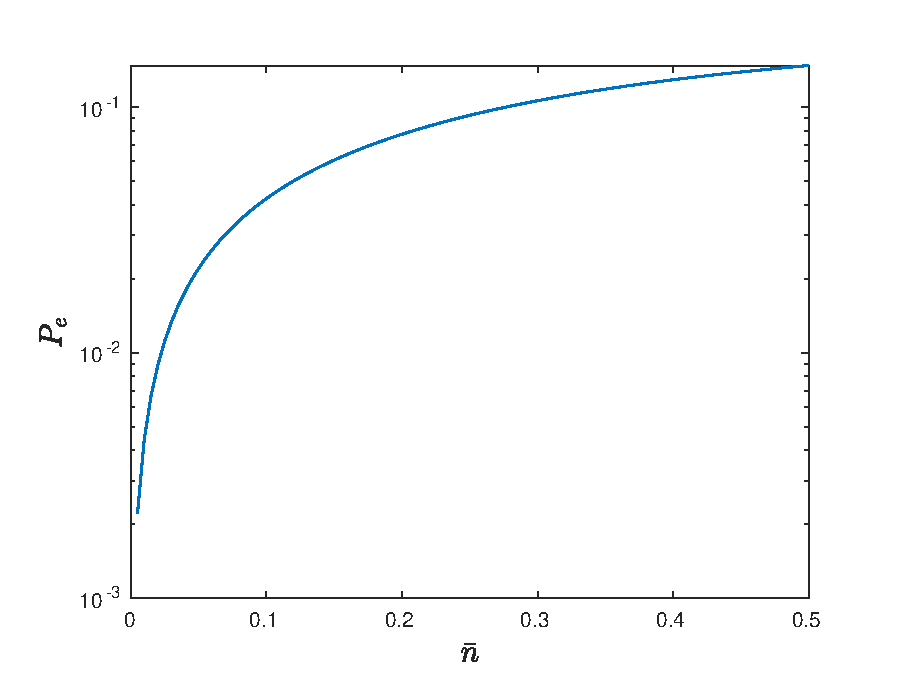
\includegraphics[width=\linewidth]{fig3.3a.eps}
            % This file was created by matlab2tikz.
%
%The latest updates can be retrieved from
%  http://www.mathworks.com/matlabcentral/fileexchange/22022-matlab2tikz-matlab2tikz
%where you can also make suggestions and rate matlab2tikz.
%
\definecolor{mycolor1}{rgb}{0.00000,0.44700,0.74100}%
%
\begin{tikzpicture}

\begin{axis}[%
width=4.521in,
height=3.566in,
at={(0.758in,0.481in)},
scale only axis,
xmin=0,
xmax=0.5,
xlabel style={font=\color{white!15!black}},
xlabel={$\bar{n}$},
ymode=log,
ymin=0.001,
ymax=0.147419865336096,
yminorticks=true,
ylabel style={font=\color{white!15!black}},
ylabel={$P_e$},
axis background/.style={fill=white}
]
\addplot [color=mycolor1, forget plot]
  table[row sep=crcr]{%
0	0\\
0.005	0.00222306458760491\\
0.01	0.00445095182430644\\
0.015	0.00667922803318255\\
0.02	0.00890374716857811\\
0.025	0.0111207871692867\\
0.03	0.0133271365234039\\
0.035	0.015520138440334\\
0.04	0.0176976872314776\\
0.045	0.0198581845006647\\
0.05	0.0220004699494153\\
0.055	0.0241237421657058\\
0.06	0.0262274812666942\\
0.065	0.0283113804877445\\
0.07	0.0303752896534372\\
0.075	0.0324191706748688\\
0.08	0.0344430637383873\\
0.085	0.0364470623029836\\
0.09	0.0384312950093298\\
0.095	0.0403959128344454\\
0.1	0.0423410801329812\\
0.105	0.0442669685051635\\
0.11	0.0461737526887799\\
0.115	0.0480616078798664\\
0.12	0.0499307080472894\\
0.125	0.0517812249275493\\
0.13	0.0536133274760063\\
0.135	0.0554271816166031\\
0.14	0.0572229501799811\\
0.145	0.0590007929543834\\
0.15	0.0607608667983887\\
0.155	0.0625033257820513\\
0.16	0.06422832133531\\
0.165	0.0659360023910981\\
0.17	0.0676265155163994\\
0.175	0.0693000050283936\\
0.18	0.0709566130953372\\
0.185	0.0725964798233494\\
0.19	0.0742197433311179\\
0.195	0.0758265398149411\\
0.2	0.0774170036065692\\
0.205	0.0789912672262207\\
0.21	0.0805494614328905\\
0.215	0.0820917152737781\\
0.22	0.0836181561343473\\
0.225	0.0851289097902105\\
0.23	0.0866241004617222\\
0.235	0.0881038508719159\\
0.24	0.0895682823081652\\
0.245	0.0910175146877452\\
0.25	0.0924516666273165\\
0.255	0.0938708555162005\\
0.26	0.0952751975931942\\
0.265	0.096664808026611\\
0.27	0.0980398009971473\\
0.275	0.0994002897831278\\
0.28	0.100746386847655\\
0.285	0.102078203927173\\
0.29	0.103395852120919\\
0.295	0.104699441980766\\
0.3	0.105989083600946\\
0.305	0.107264886707143\\
0.31	0.108526960744486\\
0.315	0.109775414963954\\
0.32	0.11101035850676\\
0.325	0.11223190048627\\
0.33	0.113440150067058\\
0.335	0.114635216540708\\
0.34	0.115817209398021\\
0.345	0.116986238397282\\
0.35	0.118142413628289\\
0.355	0.119285845571886\\
0.36	0.120416645154732\\
0.365	0.121534923799118\\
0.37	0.122640793467639\\
0.375	0.123734366702562\\
0.38	0.124815756659783\\
0.385	0.125885077137289\\
0.39	0.126942442598043\\
0.395	0.127987968187293\\
0.4	0.129021769744297\\
0.405	0.130043963808497\\
0.41	0.131054667620203\\
0.415	0.132053999115897\\
0.42	0.133042076918244\\
0.425	0.134019020320982\\
0.43	0.134984949268838\\
0.435	0.135939984332677\\
0.44	0.136884246680076\\
0.445	0.137817858041567\\
0.45	0.138740940672783\\
0.455	0.139653617312769\\
0.46	0.140556011138738\\
0.465	0.141448245717535\\
0.47	0.142330444954121\\
0.475	0.143202733037346\\
0.48	0.144065234383338\\
0.485	0.144918073576784\\
0.49	0.145761375310418\\
0.495	0.146595264322999\\
0.5	0.147419865336096\\
};
\end{axis}

\begin{axis}[%
width=5.833in,
height=4.375in,
at={(0in,0in)},
scale only axis,
xmin=0,
xmax=1,
ymin=0,
ymax=1,
axis line style={draw=none},
ticks=none,
axis x line*=bottom,
axis y line*=left
]
\end{axis}
\end{tikzpicture}%
            \caption{$k=1$ and $\mu = 0.54$}
        \end{subfigure}
        %\hspace*{fill}
        \begin{subfigure}{0.5\textwidth}
            %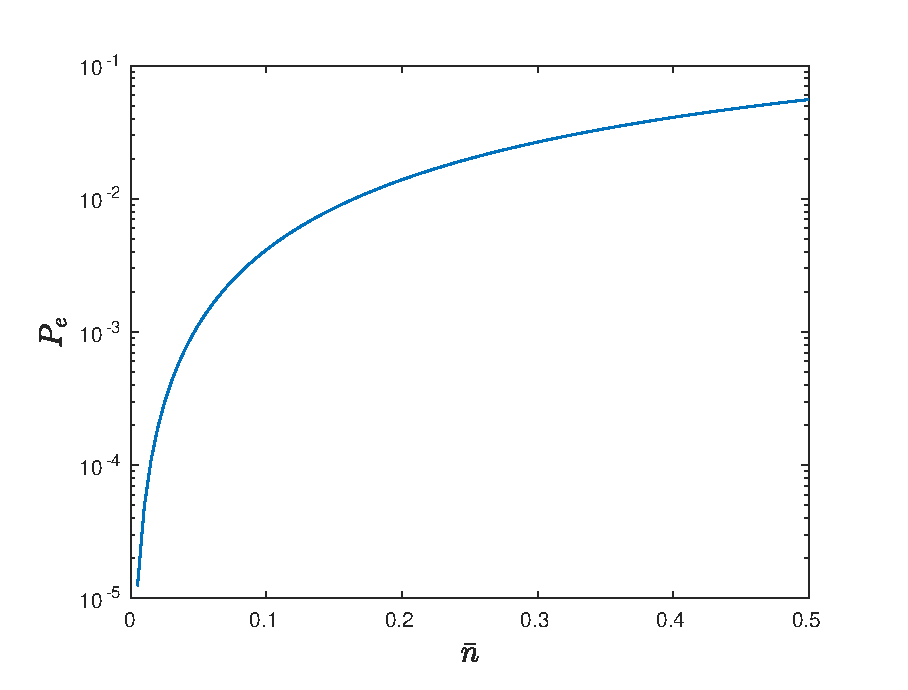
\includegraphics[width=\linewidth]{fig3.3b.eps}
            % This file was created by matlab2tikz.
%
%The latest updates can be retrieved from
%  http://www.mathworks.com/matlabcentral/fileexchange/22022-matlab2tikz-matlab2tikz
%where you can also make suggestions and rate matlab2tikz.
%
\definecolor{mycolor1}{rgb}{0.00000,0.44700,0.74100}%
%
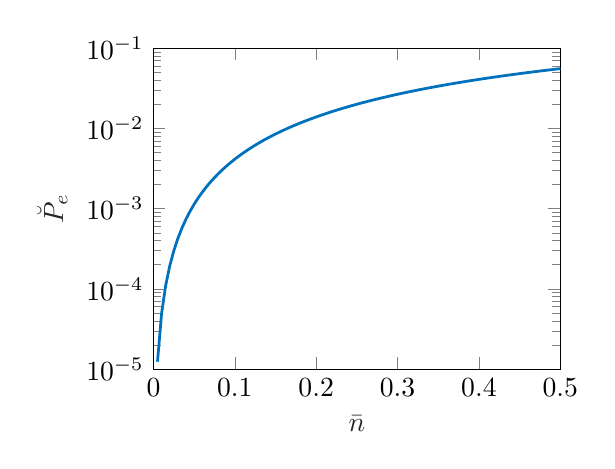
\begin{tikzpicture}

\begin{axis}[%
width=4.521in*0.45,
height=3.566in*0.45,
at={(0.758in,0.481in)},
scale only axis,
xmin=0,
xmax=0.5,
xlabel style={font=\color{white!15!black}},
xlabel={$\bar{n}$},
ymode=log,
ymin=1e-05,
ymax=0.1,
yminorticks=true,
ylabel style={font=\color{white!15!black}},
ylabel={$\breve{P}_e$},
axis background/.style={fill=white}
]
\addplot [color=mycolor1, forget plot, line width=1.0pt]
  table[row sep=crcr]{%
0	0\\
0.005	1.23759266152379e-05\\
0.01	4.90148023624126e-05\\
0.015	0.00010919944672183\\
0.02	0.000192233756247551\\
0.025	0.000297441998810322\\
0.03	0.000424168159110061\\
0.035	0.000571775303974231\\
0.04	0.000739644970414122\\
0.045	0.000927176575627686\\
0.05	0.00113378684807275\\
0.055	0.0013589092787672\\
0.06	0.00160199359202545\\
0.065	0.00186250523485199\\
0.07	0.00213992488426906\\
0.075	0.00243374797187668\\
0.08	0.00274348422496568\\
0.085	0.0030686572235552\\
0.09	0.0034088039727298\\
0.095	0.00376347448968956\\
0.1	0.00413223140495861\\
0.105	0.00451464957719938\\
0.11	0.00491031572112632\\
0.115	0.0053188280480202\\
0.12	0.00573979591836721\\
0.125	0.00617283950617264\\
0.13	0.00661758947450836\\
0.135	0.00707368666187985\\
0.14	0.0075407817790088\\
0.145	0.00801853511565381\\
0.15	0.00850661625708882\\
0.155	0.0090047038098986\\
0.16	0.00951248513674191\\
0.165	0.0100296560997625\\
0.17	0.0105559208123311\\
0.175	0.0110909913988231\\
0.18	0.0116345877621377\\
0.185	0.0121864373586856\\
0.19	0.0127462749805805\\
0.195	0.0133138425447732\\
0.2	0.0138888888888885\\
0.205	0.0144711695735268\\
0.21	0.0150604466907997\\
0.215	0.0156564886788937\\
0.22	0.0162590701424348\\
0.225	0.0168679716784675\\
0.23	0.0174829797078461\\
0.235	0.0181038863118555\\
0.24	0.0187304890738814\\
0.245	0.0193625909259528\\
0.25	0.0200000000000002\\
0.255	0.0206425294836586\\
0.26	0.0212899974804736\\
0.265	0.021942226874346\\
0.27	0.0225990451980905\\
0.275	0.0232602845059592\\
0.28	0.0239257812500001\\
0.285	0.0245953761601236\\
0.29	0.0252689141277568\\
0.295	0.0259462440929622\\
0.3	0.0266272189349113\\
0.305	0.0273116953655991\\
0.31	0.0279995338266998\\
0.315	0.0286905983894521\\
0.32	0.0293847566574839\\
0.325	0.0300818796724814\\
0.33	0.0307818418226016\\
0.335	0.0314845207535523\\
0.34	0.0321897972822458\\
0.345	0.0328975553129449\\
0.35	0.03360768175583\\
0.355	0.0343200664478965\\
0.36	0.0350346020761245\\
0.365	0.0357511841028325\\
0.37	0.0364697106931642\\
0.375	0.0371900826446282\\
0.38	0.0379122033186305\\
0.385	0.0386359785739419\\
0.39	0.039361316702034\\
0.395	0.0400881283642298\\
0.4	0.0408163265306124\\
0.405	0.0415458264206379\\
0.41	0.0422765454453999\\
0.415	0.0430084031514938\\
0.42	0.0437413211664353\\
0.425	0.0444752231455833\\
0.43	0.0452100347205243\\
0.435	0.0459456834488702\\
0.44	0.0466820987654321\\
0.445	0.0474192119347229\\
0.45	0.0481569560047562\\
0.455	0.048895265762095\\
0.46	0.0496340776881211\\
0.465	0.0503733299164807\\
0.47	0.051112962191679\\
0.475	0.0518529158287843\\
0.48	0.0525931336742138\\
0.485	0.0533335600675657\\
0.49	0.0540741408044665\\
0.495	0.0548148231004111\\
0.5	0.0555555555555532\\
};
\end{axis}

%\begin{axis}[%
%width=5.833in*0.45,
%height=4.375in*0.45,
%at={(0in,0in)},
%scale only axis,
%xmin=0,
%xmax=1,
%ymin=0,
%ymax=1,
%axis line style={draw=none},
%ticks=none,
%axis x line*=bottom,
%axis y line*=left
%]
%\end{axis}
\end{tikzpicture}%
            \caption{$k=2$ and $\mu = 1.58$}
        \end{subfigure}
        \caption{MDEP in corrispondence of MDEP zeros as function of $\bar{n}$ ($N=40$).}
        \label{fig:3.3}
    \end{figure}
    In figure \ref{fig:3.3}, the sluggish performance due to the thermal noise is clear. The plot
    shows the trend of MDEP, for zeros value of $\mu$, in function of $\bar{n}$; the used approximation
    is $N=30$. The MDEP in presence of noise is given using the expression \ref{eq:HelstromBound}.
    We can shown, using the formula \ref{eq:nbar}, that $\bar{n}$ in a real cases in near to zero, the 
    plot show the general trend of the MDEP.

    \begin{figure}[t]
        %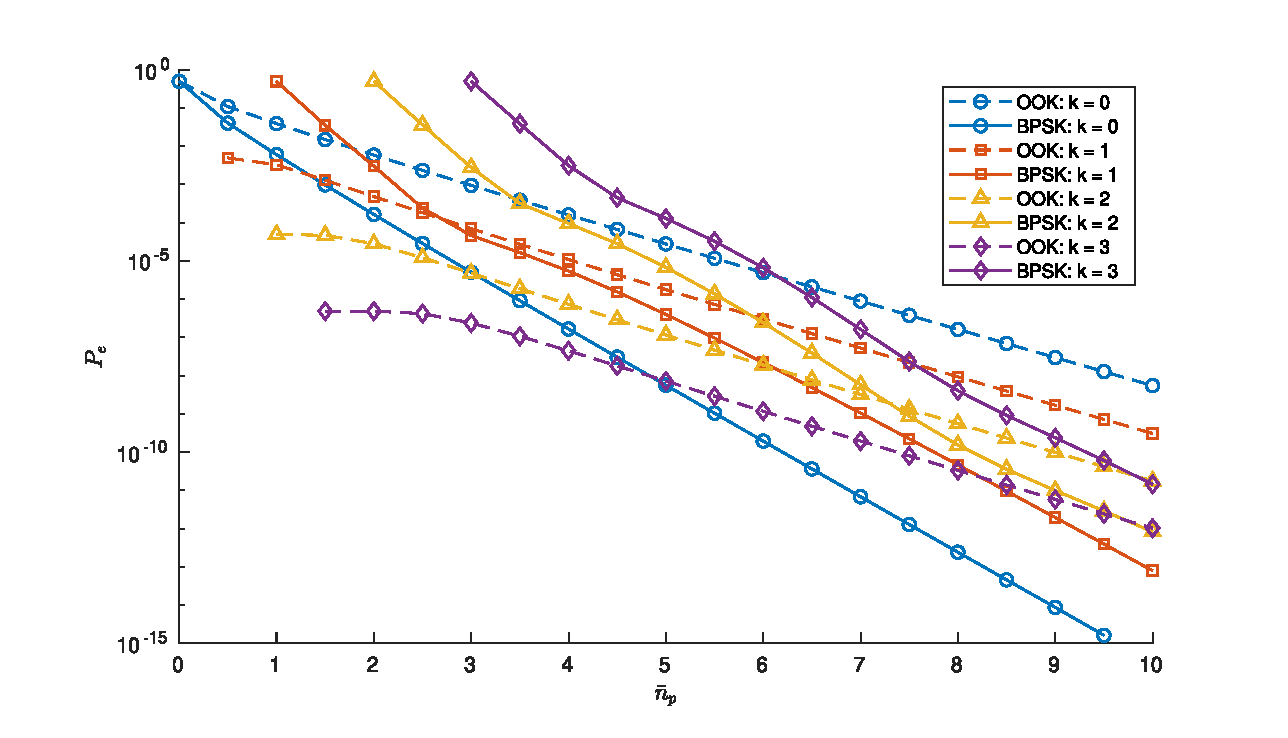
\includegraphics[width=1\textwidth]{fig3.4.eps}
        % This file was created by matlab2tikz.
%
%The latest updates can be retrieved from
%  http://www.mathworks.com/matlabcentral/fileexchange/22022-matlab2tikz-matlab2tikz
%where you can also make suggestions and rate matlab2tikz.
%
\definecolor{mycolor1}{rgb}{0.00000,0.44706,0.74118}%
\definecolor{mycolor2}{rgb}{0.00000,0.45098,0.74118}%
\definecolor{mycolor3}{rgb}{0.85098,0.32549,0.09804}%
\definecolor{mycolor4}{rgb}{0.92941,0.69412,0.12549}%
\definecolor{mycolor5}{rgb}{0.49412,0.18431,0.55686}%
%
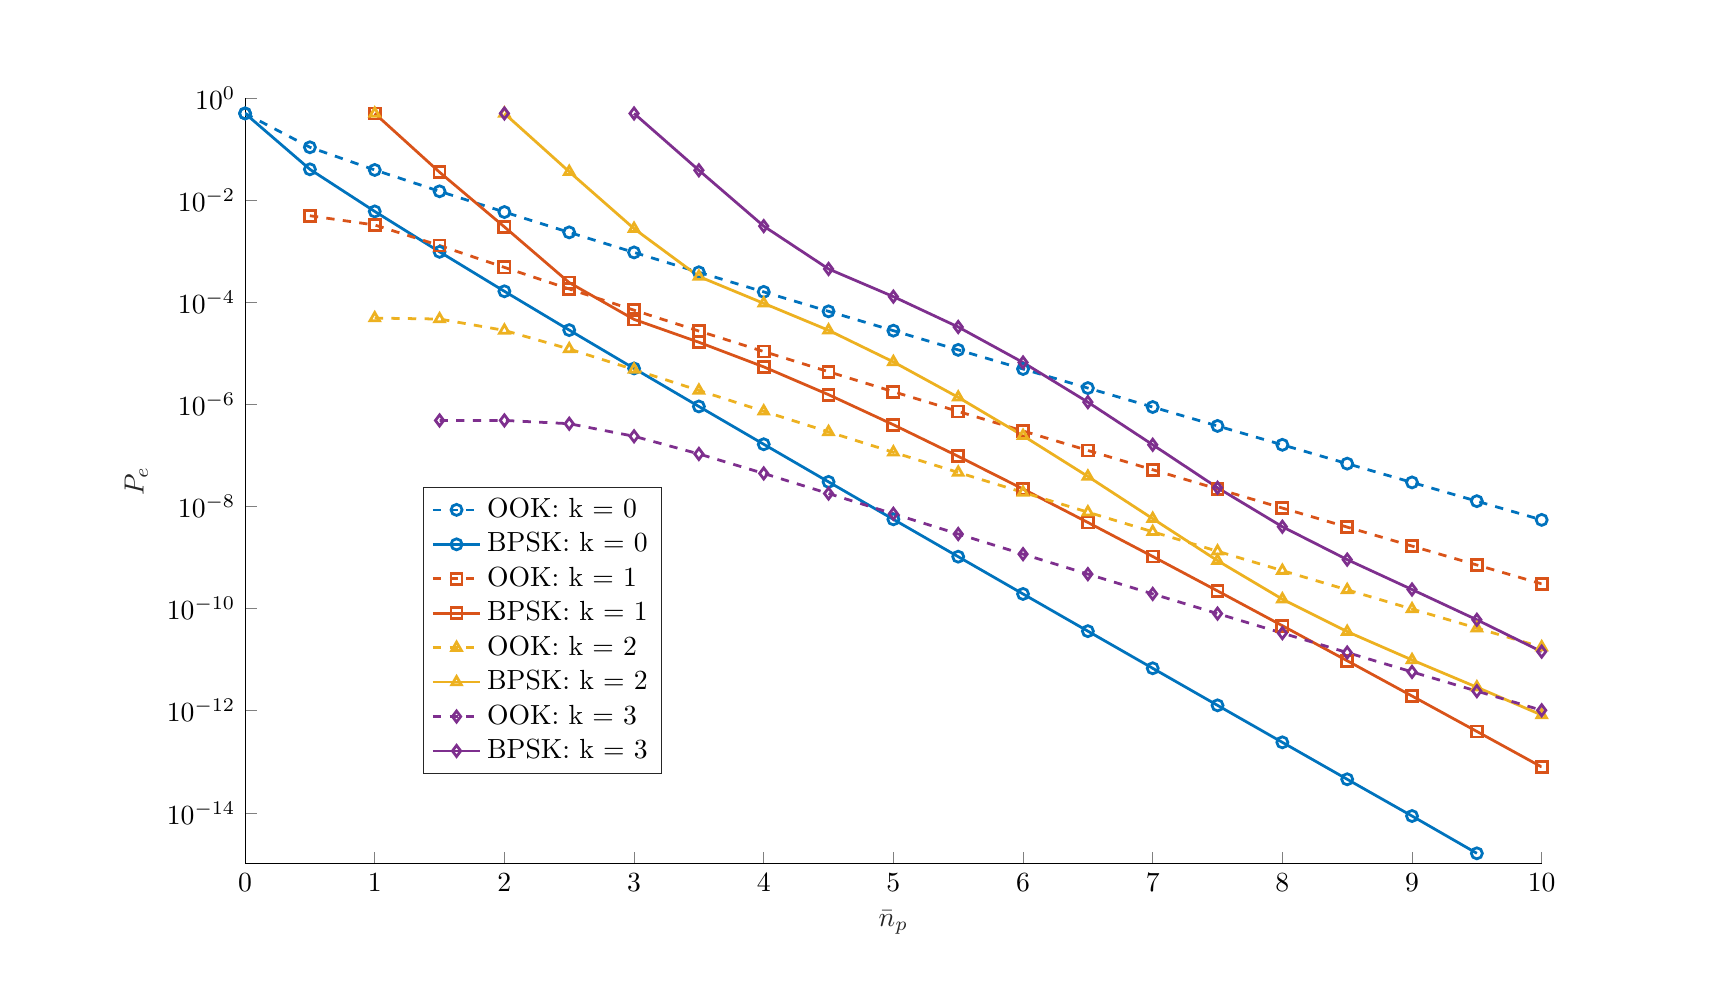
\begin{tikzpicture}

\begin{axis}[%
width=6.483in,
height=3.829in,
at={(1.087in,0.517in)},
scale only axis,
unbounded coords=jump,
xmin=0,
xmax=10,
xlabel style={font=\color{white!15!black}},
xlabel={$\bar{n}_p$},
ymode=log,
ymin=1e-15,
ymax=1,
yminorticks=true,
ylabel style={font=\color{white!15!black}},
ylabel={$P_e$},
axis background/.style={fill=white},
axis x line*=bottom,
axis y line*=left,
legend style={at={(0.137,0.117)}, anchor=south west, legend cell align=left, align=left, draw=white!15!black}
]
\addplot [color=mycolor1, dashed, line width=1.0pt, mark=o, mark options={solid, mycolor1}]
  table[row sep=crcr]{%
0	0.5\\
0.5	0.108700458264773\\
1	0.0390589952204486\\
1.5	0.0149211944183797\\
2	0.00585810811660947\\
2.5	0.00234016700918721\\
3	0.000947208632004815\\
3.5	0.000387493709571696\\
4	0.000159914025619767\\
4.5	6.64741197599072e-05\\
5	2.77990948747697e-05\\
5.5	1.1684045706617e-05\\
6	4.93169425797024e-06\\
6.5	2.08910579063692e-06\\
7	8.87685091988111e-07\\
7.5	3.78186394311975e-07\\
8	1.61491256200907e-07\\
8.5	6.90975989203757e-08\\
9	2.96172678604378e-08\\
9.5	1.27148974682356e-08\\
10	5.4664553994499e-09\\
};
\addlegendentry{OOK: k = 0}

\addplot [color=mycolor2, line width=1.0pt, mark=o, mark options={solid, mycolor2}]
  table[row sep=crcr]{%
0	0.5\\
0.5	0.04022904908515\\
1	0.00602305194817399\\
1.5	0.000973100923660764\\
2	0.00016419850351862\\
2.5	2.8533537561326e-05\\
3	5.0606940802389e-06\\
3.5	9.10735823422826e-07\\
4	1.65661779849557e-07\\
4.5	3.03786595323707e-08\\
5	5.60600271759526e-09\\
5.5	1.03974562293274e-09\\
6	1.93638272083518e-10\\
6.5	3.61866092646324e-11\\
7	6.78213041283016e-12\\
7.5	1.2740364319086e-12\\
8	2.40196751377653e-13\\
8.5	4.54081217071689e-14\\
9	8.65973959207622e-15\\
9.5	1.60982338570648e-15\\
10	0\\
};
\addlegendentry{BPSK: k = 0}

\addplot [color=mycolor3, dashed, line width=1.0pt, mark=square, mark options={solid, mycolor3}]
  table[row sep=crcr]{%
0	nan\\
0.5	0.0049504950495049\\
1	0.00326586474485618\\
1.5	0.00129261012790083\\
2	0.0004829624130685\\
2.5	0.0001823113671785\\
3	7.0042997465769e-05\\
3.5	2.73706278873798e-05\\
4	1.08587519096481e-05\\
4.5	4.36492203009786e-06\\
5	1.77428925313139e-06\\
5.5	7.28040018271869e-07\\
6	3.01099335797694e-07\\
6.5	1.25354203961425e-07\\
7	5.2479570245012e-08\\
7.5	2.20745764445418e-08\\
8	9.32266808195692e-09\\
8.5	3.95078869619425e-09\\
9	1.67926778038563e-09\\
9.5	7.15629389080874e-10\\
10	3.05683645063226e-10\\
};
\addlegendentry{OOK: k = 1}

\addplot [color=mycolor3, line width=1.0pt, mark=square, mark options={solid, mycolor3}]
  table[row sep=crcr]{%
0	nan\\
0.5	nan\\
1	0.499999999999999\\
1.5	0.0352896335380555\\
2	0.00299923864856155\\
2.5	0.000242653737939802\\
3	4.62511991632386e-05\\
3.5	1.64821131607429e-05\\
4	5.43086684001715e-06\\
4.5	1.55061238721332e-06\\
5	3.99663137751194e-07\\
5.5	9.60914410264024e-08\\
6	2.201131310553e-08\\
6.5	4.86964690793457e-09\\
7	1.04998582051152e-09\\
7.5	2.22034113317449e-10\\
8	4.6251891205884e-11\\
8.5	9.52177225954642e-12\\
9	1.94172455891817e-12\\
9.5	3.92685883809918e-13\\
10	7.91033905045424e-14\\
};
\addlegendentry{BPSK: k = 1}

\addplot [color=mycolor4, dashed, line width=1.0pt, mark=triangle, mark options={solid, mycolor4}]
  table[row sep=crcr]{%
0	nan\\
0.5	nan\\
1	4.90148024703263e-05\\
1.5	4.69619801760079e-05\\
2	2.81400977715229e-05\\
2.5	1.21516986146264e-05\\
3	4.80779255018771e-06\\
3.5	1.8744231199963e-06\\
4	7.33274078568158e-07\\
4.5	2.89379251172672e-07\\
5	1.15376949660906e-07\\
5.5	4.64708893033183e-08\\
6	1.88930928124442e-08\\
6.5	7.74504199663184e-09\\
7	3.19797588410609e-09\\
7.5	1.3287062561318e-09\\
8	5.55022250381398e-10\\
8.5	2.32915908782161e-10\\
9	9.81361103491452e-11\\
9.5	4.14942524784578e-11\\
10	1.76007541874412e-11\\
};
\addlegendentry{OOK: k = 2}

\addplot [color=mycolor4, line width=1.0pt, mark=triangle, mark options={solid, mycolor4}]
  table[row sep=crcr]{%
0	nan\\
0.5	nan\\
1	0.499999999999999\\
1.5	nan\\
2	0.499999999999999\\
2.5	0.0360954876474859\\
3	0.00276941242655876\\
3.5	0.000319766164387114\\
4	9.53611828535816e-05\\
4.5	2.83021512554327e-05\\
5	6.79567874584119e-06\\
5.5	1.37440529535127e-06\\
6	2.43371243435764e-07\\
6.5	3.88095893755214e-08\\
7	5.77702952142545e-09\\
7.5	8.68486338401198e-10\\
8	1.53136836544832e-10\\
8.5	3.53925222462692e-11\\
9	9.87959714038311e-12\\
9.5	2.88774559820126e-12\\
10	8.2261975009601e-13\\
};
\addlegendentry{BPSK: k = 2}

\addplot [color=mycolor5, dashed, line width=1.0pt, mark=diamond, mark options={solid, mycolor5}]
  table[row sep=crcr]{%
0	nan\\
0.5	nan\\
1	nan\\
1.5	4.85295073904268e-07\\
2	4.85188186849506e-07\\
2.5	4.18524906398154e-07\\
3	2.37374074729679e-07\\
3.5	1.07056314702092e-07\\
4	4.4415013722432e-08\\
4.5	1.79385606369209e-08\\
5	7.19588255648773e-09\\
5.5	2.89069451708812e-09\\
6	1.16715109799159e-09\\
6.5	4.74318695431464e-10\\
7	1.94059157632154e-10\\
7.5	7.99046939725656e-11\\
8	3.30934168957242e-11\\
8.5	1.37772571129346e-11\\
9	5.76222403125826e-12\\
9.5	2.41978659332176e-12\\
10	1.02018393732806e-12\\
};
\addlegendentry{OOK: k = 3}

\addplot [color=mycolor5, line width=1.0pt, mark=diamond, mark options={solid, mycolor5}]
  table[row sep=crcr]{%
0	nan\\
0.5	nan\\
1	nan\\
1.5	nan\\
2	0.499999999999999\\
2.5	nan\\
3	0.499999999999999\\
3.5	0.038524516196445\\
4	0.00310391579382863\\
4.5	0.000449655868986432\\
5	0.000129067667460958\\
5.5	3.28086831108965e-05\\
6	6.62678014318185e-06\\
6.5	1.10667807207143e-06\\
7	1.61993491565315e-07\\
7.5	2.33065918231468e-08\\
8	4.01583000186889e-09\\
8.5	9.11784814316974e-10\\
9	2.36422659227742e-10\\
9.5	6.03608274474254e-11\\
10	1.43704492749919e-11\\
};
\addlegendentry{BPSK: k = 3}

\end{axis}

\begin{axis}[%
width=8.365in,
height=4.698in,
at={(0in,0in)},
scale only axis,
xmin=0,
xmax=1,
ymin=0,
ymax=1,
axis line style={draw=none},
ticks=none,
axis x line*=bottom,
axis y line*=left
]
\end{axis}
\end{tikzpicture}%
        \caption{BPSK and OOK comparison in terms of MDEP as function of $\bar{n}_p$. \\$N=45$, $\bar{n}=10^{-2}$, $p_0=p_1=1/2$}
        \label{fig:3.4}
    \end{figure}
    
    The figure \ref{fig:3.4} show a comparison between a QBPSK system and a QOOK system in terms of 
    MDEP as function of $\bar{n}_p$, i.e. the mean number of photons in the system. 
    The plots are given with $\bar{n}= 10^{-2}$, $N=45$ and equiprobable symbols.
    The obtained result is really intresting: the quantum BPSK system has a sluggish performance due two 
    the photon addition process. At an equal level of energy $\bar{n}_p$, for PACS systems, it is
    possible to find an OOK configuration that maximizes the performance.
    